\section{Introduction}
%흐름
%1. 보안 업무가 점점 힘들어진다.
%2. 피쳐 엔지니어링과 머신러닝으로 보안 전문가에게 도움을 주고자 했다.
%3. 동적 피쳐는 얻기 어렵고, 정적 피쳐인 Syntactic/ structural feature 로는 시멘틱을 담기 어렵다.
%3. Semantics - aware 라는 말은, 사람이 생각하는 멀웨어 샘플들간의 관계가 담겨있다는 뜻이다. 구조적으로 다르다고 해도 멀웨어의 행위가 일치하면 같은 의미를 갖는 샘플이라고 볼 수 있다. 마찬가지로 구조적으로 거의 같다고 해도 멀웨어의 행위가 전혀 다르다면 두 샘플은 다른 의미를 가졌다고 할 수 있다. 더불어 우리는 Locky 와 Cerber 라는 두 랜섬웨어 패밀리에 해당하는 샘플 간 유사도가 Locky 와 Coinminer 에 해당하는 두 샘플의 유사도보다 더 작다고 생각한다. 이러한 샘플들 간 의미 차이 까지 담고 있는 피쳐를 Symantics-aware 피쳐 라고 할 수 있다. 
%3. 신택틱 피쳐로 시멘틱을 담아보려고 보안 전문가가 피쳐 엔지니어링을 해서 악성 행위의 구조적 패턴을 조금 더 잘 검출하는 피쳐를 획득할 수 있었지만, 복잡한 시멘틱까지 표현하는 머신러닝 모델을 만들기 위해서는 다양한 도메인에서 증명된 딥러닝같은 특징 표현 학습 기법을 멀웨어 도메인에 적용하는것을 고려해야한다.
%4. 특히 딥러닝은 전문가에 의해 피쳐 엔지니어링 된 피쳐들 뿐만 아니라, malware 바이너리, 소스코드, 메타데이터, 리소스, 동적 행위로그, 스크린샷 등 엔지니어링 되지 않은 인풋들에 대해서도 레이턴트 피쳐 표현을 배울 수 있다는 이점이 있다.
%5. 그렇다면 좋은 인풋 feature 와 딥러닝의 레이턴트 피쳐 표현 학습 능력이 있다면 멀웨어의 의미 관계까지 배울 수 있는가? 못한다. 이유는 패밀리 네이밍이 안좋아서. 그렇게 얻은 표현 레이턴트 피쳐 표현은 거의 동일한 멀웨어들은 거리가 가깝고 동일하지 않은 멀웨어들은 거리가 멀 뿐 그 거리로부터 어떤 리즈닝을 할 수 없다. 
%6. 그러면 어떻게 해야 멀웨어의 시멘틱을 딥러닝으로 학습할 수 있는가? 우리의 방법은 이러하다. 우리는 멀웨어 샘플의 의미(Semantics)를 벡터로 모델링하고 그 공간이 시멘틱 스페이스가 되도록 하였다. 그 방법으로는 첫 째, 멀웨어의 표현 벡터를 시멘틱 컴퍼넌트 벡터들의 리니어 컴비내이션이 되도록 학습하여 특정 의미를 갖게 하였다. 둘 째, 제안된 메트릭 러닝 방법을 통해 멀웨어 표현 벡터 스페이스에서 정의된 거리가 샘플들 간 의미의 차이를 반영하도록 학습하였다.
%




하루에 30만개 이상의 멀웨어가 생성되고 있고 이 숫자는 계속 늘어나고 있다. %ref
같은 기능을 하지만 해시는 다른 멀웨어들을 자동으로 제너레이션 하는 멀웨어 obfuscation 툴들의 발전 및 배포가 그 이유이다. 

반면 보안 전문가의 시간은 늘어나지 않고 있다. 보안 전문가의 업무 중 큰 부분을 차지하는 두 가지 일이 있다. 하나는 해시로 걸러지지 않은 악성코드의 카테고리를 분류하는 일이고 두 번째는 주요 악성코드에 deep dive 해서 obfuscation 방법이나 악성 행위 방법을 공부하고 후에 나올 악성코드에 잘 대응할 수 있게 하는 것이다.   

이 두 가지 주요 업무 중에서 머신러닝이 쉽게 도움을 줄 수 있는 부분은 두 번째 태스크이다. 사실상 수많은 new 악성코드들을 보안 전문가들이 하나하나 정적 혹은 동적 분석을 통해 분류하는 일은 불가능하다. 따라서 자동으로 멀웨어를 분류하는 시스템은 예로부터 많이 만들었다. PE 스트럭쳐나 콜그래프 등의 정적 피쳐를 받아서 SVM, RF, DNN 등으로 멀웨어를 분류하는 모델이 연구되어왔다.   

하지만 이렇게 만들어진 분류기의 정확도가 만족스럽지 못하거나 새로운 샘플에 대해 대응을 잘 하지 못한다면 보안 전문가는 멀웨어 분류를 위해 학습된 머신러닝 모델을 사용하고나서 그 결과를 확인해야하는 수고를 해야한다. 그리고 그 확인 과정은 비슷한 멀웨어들을 검색해주는 시스템이 구축되어있지 않다면 수고스럽고 오래 걸린다. 

따라서 classification model 을 검증하는데에 사용할 수 있으면서도 동시에 위에서 언급한 보안 전문가의 두번째 태스크인 deep dive 에도 도움을 줄 수 있는 멀웨어 IR System 에 대한 니즈가 있다.  

멀웨어 IR System 은 자연어 혹은 비젼의 IR System 과 마찬가지로 의미적으로 비슷한 멀웨어 샘플들을 랭킹하고, retrieve 해 줄 수 있는 시스템을 말한다. 따라서 우리는 멀웨어의 의미를 담을 수 있도록 멀웨어 IR 시스템을 구축해야한다. 

시스템이 Semantics - aware 라는 말은, 사람이 생각하는 멀웨어 샘플들간의 의미론적 관계가 시스템에 담겨있다는 뜻이다. 구조적으로 다르다고 해도 멀웨어의 행위가 일치하면 같은 의미를 갖는 샘플이라고 볼 수 있다. 마찬가지로 구조적으로 거의 같다고 해도 멀웨어의 행위가 전혀 다르다면 두 샘플은 다른 의미를 가졌다고 할 수 있다. 또한 샘플들 간 의미 차이 까지 고려될 수 있다면 그 시스템은 Semantics-aware한 시스템이라고 할 수 있다. 
 
Traditionally Semantic-aware Feature 를 사용해서 Semantics 를 담는 시스템을 구축하고자하는 시도가 있었다. 가장 멀웨어의 행위를 잘 나타낼 수 있는 동적 피쳐는 모든 경우의 수를 탐색하기 어렵기에 얻기가 어렵다는 단점이 있다. 정적 분석으로 얻을 수 있는 Syntatic 피쳐로 멀웨어 샘플의 의미를 표현하기 위해 보안 전문가가 피쳐 엔지니어링을 해서 특정 악성 행위의 공통적인 패턴을 조금 더 잘 검출하는 hand-crafted 피쳐를 획득할 수 있었지만, 복잡한 의미 관계까지 표현하는 머신러닝 모델을 만들기 위해서는 다양한 도메인에서 증명된 딥러닝같은 특징 표현 학습 기법을 멀웨어 도메인에 적용하는것을 고려해야한다.
 
딥러닝은 보안 전문가에 의해 피쳐 엔지니어링 된 피쳐들 뿐만 아니라, malware 바이너리, 소스코드, 메타데이터, 리소스, 동적 행위로그, 스크린샷 등 엔지니어링 되지 않은 인풋들에 대해서도 같은 의미를 갖는 멀웨어 샘플들을 표현하기 위한 공통 레이턴트 피쳐 표현을 하이러키컬하게 배울 수 있기에 Generalization 관점에서 이점이 있다. 또한 풍부한 Capacity 로 복잡한 의미관계를 학습할 수 있다는 장점도 있다. 

그렇다면 좋은 인풋 feature 와 딥러닝의 레이턴트 피쳐 표현 학습 능력이 있다면 멀웨어의 의미 관계까지 배울 수 있는가? 자연어 도메인에서는 의미 관계를 학습하기 위해서 문장에서의 앞 뒤 관계를 활용하거나[word2vec] 컨텍스트에 기반하여 co-occurence 를 확률적으로 표현한 메트릭스를 활용하는[GloVe?] 등, Self- supervised 방법을 활용한다. 하지만 멀웨어는 self-supervised learning 을 할 만한 요소가 없기 때문에, supervised learning 을 통해 의미 관계를 학습시키는 방법을 사용해볼 수 있다. 지금까지 알려진 대부분의 Deep Learning 기반 Malware Classifier는 어떤 파일이 어떤 malware family로 명명되어 있는 지를 분류하도록 가르친다. 하지만 이를 학습시켜서 얻은 representation latent feature 들은 거리가 가까우면 거의 동일한 멀웨어이고 거리가 멀면 동일하지 않은 멀웨어라는 것을 알 수 있을 뿐, 거리의 차이가 의미의 차이를 표현해주지는 않는다.  

%더불어 가르친 Malware family 가 너무 대분류라면 공통 피쳐를 학습할 수 없어서 외워버리게 되고 overfitting 하게 될 것이고 너무 소분류라면 애초에 뽑을 공통 피쳐가 없을 것이기 때문에 역시 새 샘플에 대응하기가 힘들 것이다. 
그러면 어떻게 해야 멀웨어의 시멘틱을 딥러닝으로 학습할 수 있는가? 악성 프로퍼티는 여러개이고 []. 우리는 정제된 멀티 레이블을 제공하여 딥러닝 모델이 학습할 Semantics를 지도해주었다. 그리고 멀웨어의 표현 벡터를 시멘틱 컴퍼넌트 벡터들의 리니어 컴비내이션이 되도록 학습하여 특정 의미를 갖게 하였다. 또한 우리가 제안한 메트릭 러닝 방법을 통해, 벡터 스페이스에서의 멀웨어 샘플들 간 거리가 의미의 차이와 같아지도록 학습하였다. 그리하여 멀웨어 샘플의 의미(Semantics)를 벡터로 표현할 수 있는 멀웨어 시멘틱 스페이스를 디자인할 수 있었다. 

이렇게 학습된 Semantic Space에서 의미적으로 유사한 멀웨어 또는 어떤 semantic의 차이를 갖는 malware, 혹은 특정 의미를 갖는 멀웨어들을 검색할 수 있는 유연한 IR system을 소개한다. 그리고 정량 평가와 정성 평가를 통해 시멘틱 스페이스가 얼마나 잘 만들어졌는지 확인한다.  

우리의 메인 컨트리부션은 이렇게 요약할 수 있다.

\begin{itemize}
\item 우리는 악성코드의 Semantics를 벡터로 모델링하고 어떤 악성코드의 latent feature representation을 semantic components의 linear combination으로 표현할 수 있는 Semantics Space 위에 임베딩했다. 그리고 이를 학습하기 위한 Deep Learning 기반 Malware Classifier의 구조를 제안한다.
\item 우리는 Malware Classifier가 학습하는 Semantic Space에서 metric function이 semantics의 차이를 학습하기 위해 multilabel centerloss에 기반한 Metric Learning 기법을 제안한다.
\item 학습된 Semantic Space에 존재하는 멀웨어 샘플 벡터들에 대해 멀웨어, 시멘틱, 멀웨어와 시멘틱의 조합 세 가지 방법으로 malware를 검색할 수 있는 유연한 IR system을 소개하고 그 성능을 평가한다.
\end{itemize}

페이퍼 구성은 다음과 같다. 딥러닝, IR, Metric learning, Semantic Space 등 주요 배경 지식에 대한 설명하는 Background 가 섹션 2에 위치한다. 섹션 3는 멀웨어 IR 시스템에 대한 구조와 desired properties 를 정의한다. 섹션 4에서는 우리가 학습할 멀웨어 시멘틱 스페이스를 설명하고 이를 학습하기 위한 우리의 제안을 보여준다. 섹션 5에서는 실험에 쓰인 데이터셋과 뉴럴넷 하이퍼파라미터 설정들, 그리고 정량 평가와 정성 평가 실험 결과에 대해서 설명한다. 섹션 6에서는 related works 를, 섹션 7에서는 Future works 그리고 세션 8 에서는 conclusion 이 위치한다. 

% contribution 에 centerloss 어그멘트했다고쓰기.

\section{Background}

% Handcrafted Feature Extract
\subsection{Deep learning }

 neural networks는 훈련 데이터의 통계적 특성을 기반으로 특징을 추출할 수 있는 machine learning 방법이다. 또한 DNN은 network를 수 층의 hidden layers로 구성함으로써 hierarchical feature representation을 얻을 수 있다. 일반적으로 DNN은 input layer와 수 개의 hidden layer, output layer로 구성된다. Classification task의 경우, input layer는 task의 목적이 되는 sample의 feature vector representation을 입력으로 받는다. Output layer는 주어진 input vector에 관계된 class의 probability를 vector로 출력한다. 이를 통해 DNN은 input vector에 따른 class를 predict 할 수 있다.
 
특히 Image classification task의 경우 Convolutional network를 사용함으로써 모델의 성능을 향상시킬 수 있다.[ref?] Convolutional network는 convolutional layer와 pooling layer, 일반적인 neural network layer로 구성되며, convolutional layer의 경우 filter를 input에 대해 convoluting함으로써 feature를 추출한다. Pooling layer의 경우 영향을 적게 주는 feature를 down sampling하는 효과를 얻는다.


\subsection{Information Retrieval}
Information retrieval 은 본래 유저의 string  쿼리로부터 관련 문서를 찾는 태스크로 자연어 처리 분야에서 발전하였다. 하지만 이를 다른 도메인으로 확장시켜 이미지\cite{datta2008image, yu2015learning}, 음악\cite{schedl2014music}, 의료\cite{goeuriot2016medical, mourao2015multimodal}, 멀웨어\cite{santos2013noa} 등 다양한 분야에서 사용되고 있다. 

\textbf{Boolean Model. }Information Retrieval System 을 만들기위한 모델로, Boolean model 이 제안되었다. boolean model 은 boolean 로직과 집합 이론을 배경으로 하여 문서들과 유저의 쿼리들을 집합으로 대하고 검색을 시행하는 모델이다. 이는 직관적이고 구현하기 쉽다는 장점이 있었지만, 유사도가 Discrete 하게 계산되어 리트리벌 결과가 아주 많아지거나 정확히 일치하지 않으면 검색되지 않는 현상이 일어나고, 모든 term 들이 똑같은 비중을 가지는 한계들이 있었다.\cite{lashkari2009boolean, } 


\textbf{Vector Space Model.} 또 다른 방법으로 Vector space model 이 있다. 이는 문서들과 유저의 쿼리를 모두 벡터스페이스에서 표현함으로써 벡터 간 거리가 곧 유사도가 되도록 하는 모델이다. 선형 대수에 기반한 간단한 모델로, 텀에 대한 가중치를 다르게 줌으로써 리트리벌 결과를 더 좋게 만들 수 있고, 쿼리의 유사도를 continuous Value 로 나타낼 수 있다는 장점이 있다.\cite{salton1975vector} 문서와 유저의 쿼리를 벡터로 만드는 방법\cite{}과 벡터 간 거리를 측정하는 방법\cite{}에 따라 여러가지 모델들이 존재한다.


%\texttt{
%\begin{itemize}
%\item Exact matching may retrieve too few or too many documents
%\item hard to translate a query into a boolean expression
%\item all terms are equally weighted
%\item more like data retrieval than information retrieval
%\end{itemize}}



%\begin{itemize}
%\item Simple model based on linear algebra
%\item Term weights not binary
%\item Allows computing a continuous degree of similarity between queries and documents
%\item Allows ranking documents according to their possible relevance
%\item Allows partial matching
%\end{itemize}


\textbf{Learn Vector Representation Using Deep Learning.} 앞서 설명했듯, 딥러닝을 사용하여 머신러닝 태스크를 수행하면 hierarchical representation 을 배울 수 있기 때문에 Generalization 이 더 잘 되는 장점이 있다. 따라서 Vector space model 을 이용하는 여러 태스크들과 딥러닝은 조합이 좋았고, 이로인해 많은 태스크에서 성능 상 breakthrough 를 이루어냈다.[refs : imagenet, word2vec, speech recognition, ...]. 더불어 Vector space model 을 사용하는 IR 분야 또한 딥러닝과 만나면서 한번 더 Breakthrough를 이루어냈다.[refs : document retrieval, Retrieval based QA, Image retrieval]. 

벡터 representation 을 학습시키는 방법으로는 supervised 와 unsupervised 가 있다. Unsupervised 로 가르치는 대표적인 방법은 Autoencoder를 이용하는 것으로, 이를 활용해서 멀웨어를 인코딩하려는 시도[ref]가 있었다. Supervised 로 가르치는 방법은 인간이 레이블을 주고 그 레이블로의 Classification 혹은 Regression 태스크를 수행하는 딥러닝 모델을 만들어, 정보를 가장 압축적으로 담고있는 bottleneck layer 의 아웃풋을 해당 샘플의 representation vector 로 보는 것이다. 이 방식은 vector representation 의 위치를 가르치는 사람이 어느정도 컨트롤 할 수 있게 된다. 예컨데 메트릭 러닝을 위한 objective function 을 사용해서 어떤 샘플들을 가깝게 보내고 어떤 샘플들을 멀게 보낼지를 결정할 수 있고[siamese, triplet, centerloss ...], 이는 one shot or few-shot learning 의 태스크를 수행할 수 있기 때문에, 벡터 간 distance 를 기준으로 랭킹을 결정하고 적은 샘플에도 대응할 수 있어야 하는 information retrieval 의 성능을 향상시킬 수 있다. 


\subsection{Metric Learning}


\subsection{Semantic Spaces}


\section{Malware Information Retrieval System}
% 목표하는 바
이번 세션에서는 제안된 malware information retrieval system 의 동작과 구성 그리고 가져야하는 속성들을 설명한다. 우리의 시스템은 크게 학습과 검색(retrieval), 두 페이즈로 나뉜다. 학습 페이즈에서는 원할한 검색을 위해 시멘틱스를 반영하는 학습 데이터의 표현 벡터를 학습한다. 검색 페이즈에서는 유저로부터 입력된 멀웨어 혹은 태그 쿼리와 미리 저장해놓은, 학습된 표현 벡터들로부터 랭킹 결과를 출력한다. 이어지는 서브 섹션에서는 두 페이즈에서 사용될 노테이션들을 정의하고, 이들을 이용해서 각 페이즈에서 어떤 태스크를 행해야하는지를 자세히 설명한다.  


\subsection{Notations}
우리는 먼저 학습 멀웨어 셋으로 $X = \{x_1, x_2, ..., x_N\}$ 를 갖고있다. 그리고 각 멀웨어에 해당하는 싱글레이블 셋 $Y_s = \{y_{s1}, y_{s2}, ..., y_{sN}\}$ 과 멀티레이블 셋 $Y_m = \{\vec{y}_{m1}, \vec{y}_{m2}, ... , \vec{y}_{mN}\}$ 이 있다. 이 레이블을 얻는 방법은 섹션 6.1에서 설명한다. 그리고 각 멀웨어로부터 손으로 추출된 피쳐들의 셋을 $V = \{v_1, v_2, ..., v_n \}$ 로 정의한다. 

멀웨어 IR 시스템은 $[h, E, d, R]$ 4개의 원소를 갖는 tuple 로 정의된다. $h$ 는 멀웨어 피쳐로부터 벡터 representation 을 얻을 수 있는 임베더 함수이다. $E$ 는 검색이 될 멀웨어의 임베딩 벡터 셋이다. $d$ 는 입력된 쿼리와 임베딩 벡터 간 거리를 계산하는 함수이다. $R$ 은 랭킹 모듈이다. 학습 페이즈에서는 적절한 $h$ 를 학습하고 이를 통해 $V$로부터 $E$를 얻는다. 리트리벌 페이즈에서는 멀웨어 샘플 쿼리 $q$ 를 입력받고 가장 가까운 $k$ 개의 neighbor 를 랭킹 모듈 $R$ 을 통해 반환한다.

\begin{table}[!htb] % notation
\caption{Notations}
\label{tab:notation}
\begin{minipage}{\columnwidth}
\begin{center}
\begin{tabular}{ll}
\toprule
Meaning & Notation\\
\midrule
  Set of malwares     & $X$ \\
  ith malware sample  & $x_i$ \\
  Set of single labels & $Y_s$ \\
  Single label of ith malware    & $y_{si}$ \\
  Extracted features of ith malware & $v_i$ \\
  Set of extracted features   & $V$ \\
  Set of multilabels   & $Y_m$ \\
  Multilabels of ith malware & $\vec{y}_{mi}$\\
  Neural embedder & $h$ \\
  Parameters of neural embedder & $\theta$ \\
  Classifier & $g$ \\   
  Parameters of classifier & $W$, $b$ \\  
  Set of Embedded malware vectors & $E$ \\
  Embedded malware vector & $e$ \\
  Importance coefficient & $c$ \\
  Distance measuring function & $d$ \\
  Semantic component vector & $s$ \\
  Ranking Module & $R$\\
\bottomrule
\end{tabular}
\end{center}
\bigskip\centering
\end{minipage}
\end{table}


\subsection{Tasks}
학습페이즈에서는 IR system 에서 사용하기 위한 벡터 리프레젠테이션을 얻기 위한 Auxiliary Task를 수행한다. Auxiliary Task 는 멀웨어 분류 태스크를 학습하는 것으로 싱글 레이블 클래시피케이션이나 멀티레이블 클래시피케이션이 될 수 있다. $f: V \rightarrow Y $ 인 f 는 멀웨어 피쳐로부터 레이블을 추정하는 함수이다. 함수 $f$ 는 다시 $g$ 와 $h$ 의 합성 함수로 정의할 수 있다. $h$ 는 위에서 설명한, 멀웨어 피쳐로부터 vector representation 을 얻을 수 있는 임베딩 함수이다. $g$는 임베딩으로부터 label 을 추정할 수 있는 클래시파이어이다. 시멘틱을 내포하는 임베딩 벡터를 학습시키는 방법에 대해서는 섹션4에서 자세히 이야기한다. 
\[
f(v_i) = (g \circ h)(v_i) = g(h(v_i)) = g(e_i) = y_i 
\]
where
\[
g(e_i) = \sigma (W*e_i + b) 
\]
% sigma == sigmoid or softmax
리트리벌 페이즈에서는 멀웨어 샘플 쿼리 q를 입력받아 학습 페이즈에서 구했던 h 함수를 이용하여 임베딩한다. 임베딩된 쿼리 eq 와 E 의 원소들 간 거리를 d 함수를 통해 측정하고, 가까운 k 개의 neighbor 를 랭킹 모듈 R 을 통해 반환한다. 

% Algorithm 으로 대체
\[
Results = \{x_j | j = argmin_i( {-d(e_q, e_i)} )  \}
\]


\subsection{Modules}
두 페이즈의 구조도는 Figure 과 같다. 두 페이즈에서 공통으로 존재하는 모듈은 Feature Extractor와 Neural Embedder 가 있다. 벡터 학습 페이즈에는 Classifier 가, 리트리벌 페이즈에는 랭킹 모듈이 포함되어있다. 

\begin{figure}[!htb] % train_phase
  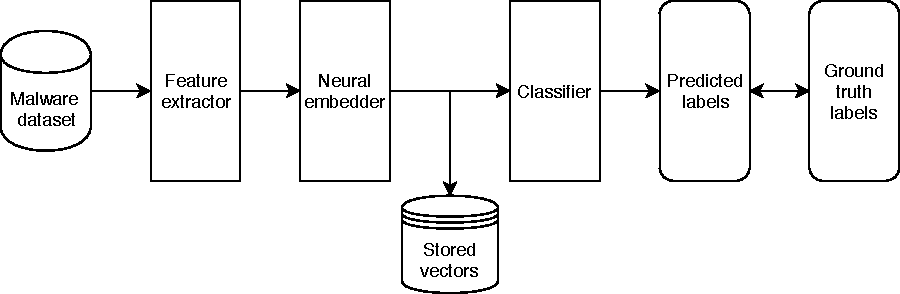
\includegraphics[width=\linewidth]{../figures/train_phase.pdf}
  \caption{train phase}
  \label{fig:train_phase}
\end{figure}

\begin{figure}[!htb] % retrieval_phase
  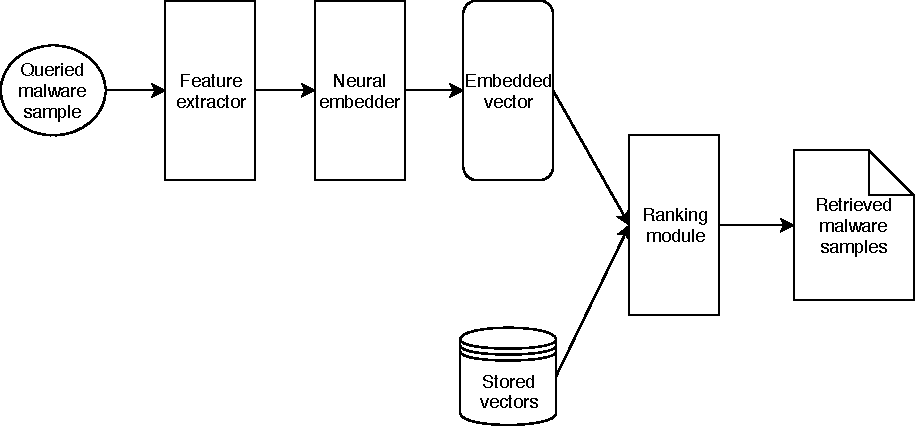
\includegraphics[width=\linewidth]{../figures/retrieval_phase.pdf}
  \caption{retrieval phase}
  \label{fig:retrieval_phase}
\end{figure}

\textbf{Feature Extractor. }
Feature extractor 는 Malware Rawdata 로부터 Handcrafted feature 를 추출하는 모듈이다. Handcrafted feature로 PE 같은경우에는 Size 와 Entropy, Histogram of API Calls, … 등을[*] 추출한다. APK 같은 경우에는 추가적으로 Permission,  … 등의 피쳐를 추출한다. 

\textbf{Neural Embedder. }
Neural embedder 는 Feature extractor 모듈에서 추출된 멀웨어의 피쳐들로부터 Representation vector 를 뽑는 모듈이다. theta 로 Parameterized 되어있는 뉴럴 네트워크이며, 파라미터는 벡터 학습 페이즈에서 Auxiliary Task 를 수행하면서 Optimize 된다. 그리고 리트리벌 페이즈에서 파라미터는 freeze 되어 업데이트되지 않는다. 
Neural Embeder 의 네트워크 구조는 CNN을 사용하였다. Thumbnail 을 받아서 CNN 5 층과 fully 2 층을 쌓은 구조를 사용한다. feature 의 성격에 따라 다른 네트워크 구조로 임베딩 피쳐벡터를 추출함으로써 더 나은 generalization 성능을 얻을 수 있다. thumbnail 피쳐는 [malimg 논문 인용] 악성 코드영역 혹은 악성코드를 특징짓는 영역의 로컬리 시프트 인베리언트한 특성을 담기 위해 CNN 을 사용해서 임베딩 피쳐벡터를 추출한다. 

\textbf{Classifier. }
%% Figure
%\begin{figure}
%  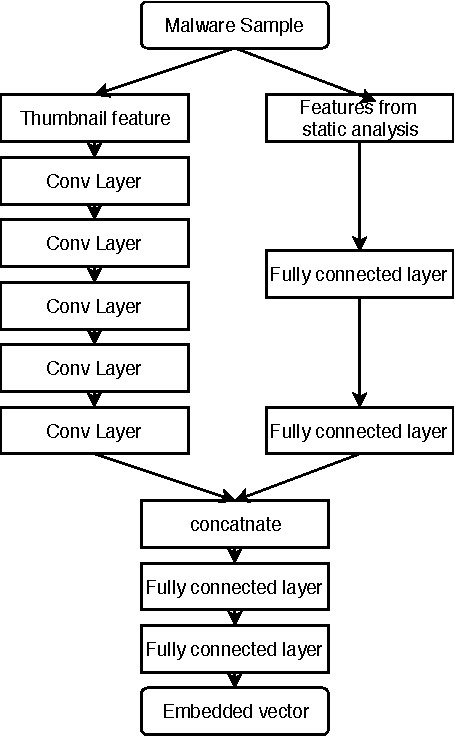
\includegraphics[height=10cm]{../figures/neural_embedder.pdf}
%  \caption{neural embedder}
%  \label{fig:three}
%\end{figure}
Classifier 모듈은 Neural embedder 를 통과해서 나온 embedding vector 를 받아서 각 레이블 별 확률을 출력해준다. 1층의 fully connected 로 파라미터라이즈드 되어있으며 태스크에 따라 softmax 혹은 sigmoid Activation을 사용하였다. Neural Embeder 모듈과 마찬가지로 벡터 학습 페이즈에서 back propagation 에 의해 파라미터들이 학습되고, 리트리벌 페이즈에서는 프리즈된다. 

\textbf{Ranking Module. }
학습 페이즈에 저장해두었던 학습 셋의 임베딩 벡터들과 추출된 벡터의 거리를 거리함수 d 를 사용하여 측정하고 k 개의 nearest neighborhood 를 가까운 순서대로 정렬하고 출력한다.


\subsection{Desired properties}
멀웨어 IR 시스템은 한계들이 존재했다. 특히 Raw binary file 로부터 좋은 피쳐를 뽑기가 수월하지 않고, intraclass variance 는 크고 innerclass variance 는 작으며 계속해서 변종과 새로운 종이 생겨나는 멀웨어 도메인의 특징으로 말미암아 좋은 멀웨어 IR 시스템이 가져야 할 속성들은 다른 도메인의 IR 시스템과는 조금 다르다.

\textbf{Semantic understanding. }
쿼링 샘플에 대해 구조적으로 비슷한 샘플 뿐만 아니라 의미적으로도 비슷한 샘플들을 랭킹하고 retrieve 할 수 있어야 한다. 여기서 의미가 비슷하는 것은 멀웨어의 행동 혹은 사람이 생각하기에 중요한 멀웨어의 속성들이 비슷하다는 것을 의미한다. 구조적으로 다르다고 해도 멀웨어의 행위가 일치하면 같은 의미를 갖는 샘플이라고 볼 수 있다. 마찬가지로 구조적으로 거의 같다고 해도 멀웨어의 행위가 전혀 다르다면 두 샘플은 다른 의미를 가졌다고 할 수 있다. 더불어 우리는 Locky 와 Cerber 라는 두 랜섬웨어 패밀리에 해당하는 샘플 간 유사도가 Locky 와 Coinminer 에 해당하는 두 샘플의 유사도보다 더 작다고 생각한다. 이러한 샘플들 간 의미 차이 까지 고려될 수 있다면 그 시스템은 Symantics-aware한 시스템이라고 할 수 있다. 
 
\textbf{Robustness to novel samples. }
멀웨어의 새로운 변종들은 계속해서 나타나기 때문에 이에 빠르게 대응할 수 있어야 한다. 
%
%\textbf{Robustness to rare inputs. }
%멀웨어 도메인에서의 샘플 수는 그 멀웨어 패밀리의 영향력을 의미하지 않는다. 물론 비례하는 경향이 없는것은 아니지만, 하나의 멀웨어가 전세계적으로 유행할 수도 있고, 변종은 많지만 별로 영향력이 없는 멀웨어일 수도 있다. 따라서 해당 패밀리의 샘플 수가 적다고해서 쿼링 결과에서 랭킹 순위가 밀려서는 안된다. 즉 적은 수의 샘플에 대해서도 모델은 강건해야한다. 

%\textbf{Robustness to variable size inputs. }
%멀웨어의 raw file size Variance 는 매우 크다. 작게는 몇키로바이트부터 크게는 기가단위까지 갈 수 있다. 사이즈에 상관없이 retrieve 를 할 수 있어야 한다.

\textbf{Efficiency. }
세상에 존재하는 멀웨어 샘플 개수는 매우 많고 기하급수적으로 늘어나고 있다. 따라서 수많은 샘플들에서 k 개의 상위 랭크된 결과를 적절한 시간 내에 retrieve 하려면 랭킹 모듈이 효율적이어야한다.




\begin{figure*}[!htb] % concept
  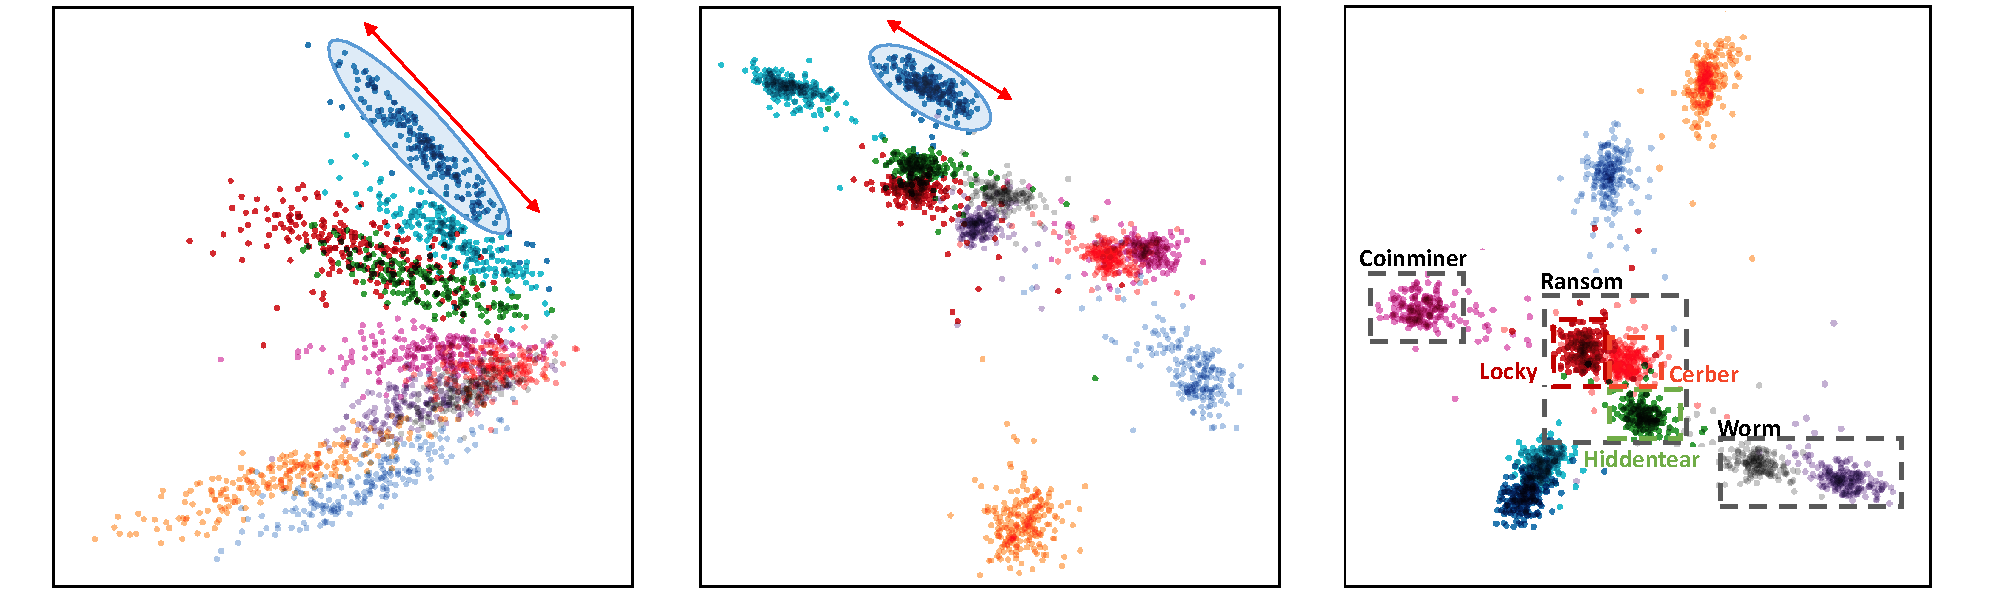
\includegraphics[width=\textwidth]{../../figures/concept.pdf}
  \caption{The concept of our proposed method. Left figure shows PCA plot of representation vectors which are trained by single label classificaion task. Center figure shows the vectors trained by training single label classification task with centerloss. We observe that of center figure's intra-class variance model is smaller than left figure's.
  Right figure shows the vectors which are trained by multi-label classification task with multi-label centerloss. It shows that representation vectors whose semantics are simliar are nearly located then others. 
%  
%  왼쪽 그림은 그냥 싱글레이블 클래시피케이션 태스크를 학습해서 얻은 리프레젠 테이션 벡터의 PCA plot이다.
%  	가운데 그림은 싱글레이블 클래시피케이션 태스크를 센터로스를 적용하여 학습해서 얻은 리프레젠테이션 벡터의 PCA plot 이다. 왼쪽 그림에 비해서 intra class variance 가 줄어들었을을 그림에서 확인할 수 있다. 오른쪽 그림은 multilabe 클래싶피케이션 테스크를 센터로스를 적용해서 학습해서 얻은 리퍼르제네테이션 벡터의 Pca plot이다. 왼쪽과 가운데 그림에 비하여 semantically similar sample의 벡터들이 가깝게 위치하였음을 확인할 수 있다. 
  }
  \label{fig:concept}
\end{figure*}

\section{Semantics Aware Representation Learning}
This section describes how the space in which malware is embedded approximates the semantic space. First, we describe malware semantic space and we propose a loss function for training semantic-aware malware representation vectors.

\subsection{Semantic Spaces for Malwares}

\textbf{Definition. }
Let $X = \{x_1, …, x_n, …, x_N\}$ be a set of malwares.
Let $S$ be a subset of vector space $V$ of dimension $d$ and let semantic component set $S = \{s_1, ... , s_k, … s_K\}$ be a linearly independent subset of $V$.  
Then for every $\mathbf{e} \in E$, there is an unique linear combination of the sementic component vectors that equals $e$.
\[
\mathbf{e} = c_1\mathbf{s_1} + c_2\mathbf{s_2} + … + c_k\mathbf{s_k} 
\]

where $c_i$ is the i’th element of coefficient vector $ \mathbf{c} = \{c_1, ... , c_k\}$ and we call it as importance coefficents.
We call a vector $\mathbf{e}$ as a semantic vector of malware $x$ and there is a nonlinear mapping from $X$ to $E$. 

\textbf{Metric function. }
we use an Euclidean Distance $d(\mathbf{e_i}, \mathbf{e_j})$ for a metric of a set E and it means the function that defines a distance between  semantics of two malwares. 

\textbf{The meaning of approximate semantic space of malwares}
We now take an example of language, thinking of the meaning of certain words. We consider the relationship of those meanings. We can assume that city names and words related to machine learning are located far away from each other. We can also imagine that the words will be near. The similarity of the relationships between words can thus be considered. The relationship between ``King’’ and ``Queen’’ is similar to the relationship between ``Man’’ and ``Woman.’’ To maximize the meanings of these words, we represent them as vectors on a vector space. If the meaning is similar, the distance between the vectors is near. If the meaning is disparate, the distance between the vectors is far away. We also approximate the semantic relationship between words by using operations defined in the vector space, such as ``king - queen = man - woman.’’


Similarly, we can imagine the semantic meaning of malicious code. We consider malware a combination of malicious components. We also use the concept of basis and linear combination to approximate it as a vector space operation. In other words, we can approximate the semantic space by training the semantic vector of malware to be represented as a linear combination of the semantic component vector.


\textbf{Evidences. } 
If we approximate the semantic space well, then the following querying tasks should work correctly. First, we should be able to retrieve semantically similar malwares by querying malware samples. Second, it should be possible to retrieve by only a combination of semantic components. For example, we should be able to retrieve malwares with these three attributes: ``ransom’’, ``downloader’’, and ``agent’’. Finally, we should be able to retrieve related samples by querying a combination of samples and semantic components such as a sample with attributes ``ransom’’ and ``downloader’’ combined with semantic component ``agent’’.


\subsection{Solution Overview}
\begin{figure*}[!htb] % qualitative_all
  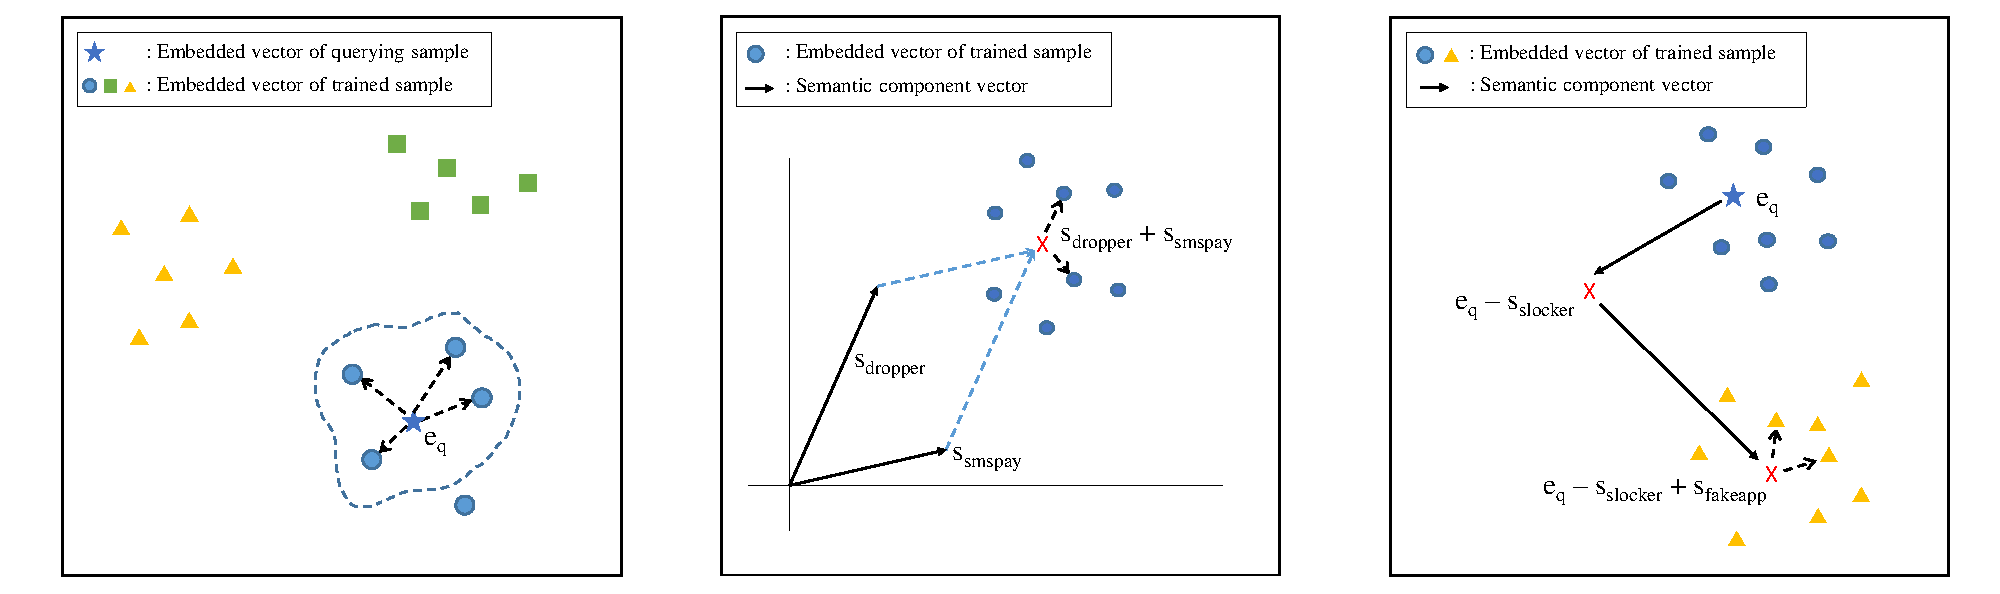
\includegraphics[width=\textwidth]{../../figures/qualitative_all_fix.pdf}
  \caption{Our malware retrieval system was queried in three ways: malware samples(left), semantic components(center) and a combination of malware samples and semantic components(reight).}
  \label{fig:qualitative_all}
\end{figure*}

\textbf{Multilabel classification. }
To train the vector representation, $E$, that reflects the meaning of the malware sample, multi-label classification learning was selected as the auxiliary task. To train this classification task, the neural embedder, $h$, places the representation vectors so that they can be classified by the linear classifier. Most studies that train malware classifiers learn classifiers to classify malware under single label.

However, if you identify a label in a malware domain and create a malware IR system based on it, then the trained embedding vector is insufficient to include the meaning of the sample. Typically, the process of labeling malware is irrational in expressing the meaning of malware. Malware often displays multiple malicious behaviors at the same time. However, existing malware labeling systems do not reflect these attributes. Additionally, naming rules are often globally inconsistent, and even locally, analysts name via differing criteria. Regarding non-prevalent malware, when one labels malware, a name is provided unrelated to the malware’s behavior. These labeling processes prevent the machine learning model from learning the appropriate meanings. 

We use the auxiliary task to classify the labels into multiple labels, and we use vector representations from the auxiliary task to enable retrieval of malware samples of similar meanings.



\textbf{Centerloss. }
To allow the representation vectors of malwares to exist on the semantic space while training multi-label classification in the above way, we use multi-label centerloss. Once in the background, the effect of centerloss is lowering the intra-class variance. This causes centerloss to prevent the intra-class variance from becoming too large and the distance between two samples in the same class to be greater than the distance between two samples of different classes, resulting in improved IR results.

Second, we can locate representation vectors to approximate the semantic space. In the paper proposing a single label centerloss, the template vector is stored in the external memory for each label, and the mean square error (MSE) is set so that the distance between the template vector and the representation vector of sample becomes small. As a result, the representation vector of the sample and the template vector of the class are approximated. Likewise, we store vectors for each semantic component in external memory, and we set the MSE error to a loss function so that representation vector is a linear combination of semantic component vectors.



%그리고, 보틀넥과 시멘틱 컴포넌트들의 합의 차이에 alpha/the number of answer labels 만큼의 곱을 하여 각 레이블을 업데이트해준다. 알파는 하이퍼파라미터로, 템플릿 벡터와 보틀넥을 얼마나 섞어서 기존 템플릿벡터를 업데이트할지를 결정해주는 값이다. 

\textbf{Learn to rank. }
In malware labels, there are important labels and those that are not. Considering this importance in creating a MR system is one of the important factors to satisfy the semantic understanding property. For example, in PE format labels, ranking more than labels such as ransom and coinminer rather than agent or downloader would be considered as a semantics-aware search system. To solve this problem, we use weighted centerloss which reflects the importance of labels with constraint. The constraint determines the norm of the semantic components. Euclidean distance, the metric function that we use in retrieval, is affected by the norm of the two vectors when computing distances. The distance between semantic component vector, having a large norm and another component vector is likely to be larger than the distance between component vectors having a small norm. Therefore, in the MR system ranking with Euclidean distance, when malware having a semantic component with a high importance is queried, the malware samples, including the semantic component, are more likely to be searched. This can be regarded as a scoring technique (i.e., tf-idf\cite{baeza1999modern}), making it possible to search documents with specific properties more easily in the existing information retrieval system.
 


\subsection{Proposed Objective Functions}
We propose a new objective function to learn the semantic space by the methods described in the Section 4.2.

\textbf{Multi-label center loss(MCL). }
The expression of the constrained optimization problem we want to solve is equal to Eq.\ref{eqn:optimization}. This adds a constraint that the distance between the target semantic vector and the representation vector should be less than $\epsilon$ on the negative log likelihood optimization problem, which is the basis of the cross-entropy loss.



\begin{equation}
\label{eqn:optimization}
\min_{\theta, W, \mathbf{b}} J(\theta, W, \mathbf{b}) = -\sum_i{ \sum_j{ y_{mij} \log{\hat{y_{ij}}}}}
\end{equation}

s.t.
\[
h(v_i;\theta)) - \mathbf{s}_\text{target} < \epsilon ,
\]
%\[
%||c_i||_2 = cc_i
%\]
for $i \in \{1,2, ..., N\}$ where $\epsilon >= 0$ and $s_\text{target}$ is a target semantic vetcor.

To find the parameters satisfying the above equation, the final loss function was constructed by adding cross-entropy loss and multilabel centerloss at a ratio of 1:$\lambda$\cite{wen2016discriminative}. We can formulate the loss function we propose as Eq.\ref{eqn:centerloss}. 

\begin{equation}
\label{eqn:centerloss}
\begin{aligned}
L &= L_s + \lambda L_c \\
 &= -\frac{1}{N}\sum_i{\sum_j{ y_{mij} \log{\hat{y_{ij}}}}} 
+ \lambda \frac{1}{N} \sum_i{( \mathbf{s}_{\text{target}} - h(v_i;\theta))^2}\\
\end{aligned}
\end{equation}

where 
\[
\hat{y_{ij}} = \frac{\exp(Wh(v_i;\theta)+\mathbf{b})}{ 1 + \exp(Wh(v_i;\theta)+\mathbf{b})}
\]

%$L_c = \sum_i^N{||e_i - s_\text{target}||^2}$

  
\textbf{Weighted multi-label center loss(WMCL). }
As described above, we apply importance coefficients for each semantic component to apply the learn to rank technique to our Malware Information Retrieval System. We added a constraint such that the importance coefficient value is equal to the norm of the semantic component vector. 

\[
||\mathbf{s_i}|| = c_i \text{ for all i }\in \{i = 1,2, ..., M\}
\]

The cross-entropy loss updates the parameters of $ \theta, W, \mathbf{b} $ to improve the accuracy of multilabel classification. Multi-label centerloss updates parameters as follows. First, the parameters of $\theta, W, \mathbf{b} $ are updated so that the embedding vector is close to $\mathbf{s}_{\text{target}} $ via back propagation. Second, the semantic components are updated so that $ \mathbf{s}_{\text{target}} $ is close to the embedding vector. When updating, we divide difference vector between $\mathbf{s}_{\text{target}}$ of current step and embedding vector equally and we add it to each semantic component vectors, such that $\mathbf{s}_{\text{target}}$ of next step to be locate at Internally dividing point of current $\mathbf{s}_{\text{target}}$ and embedding vector of sample. 

There are several methods to combine semantic component vectors, we propose summation model and average model. The performance of each model can be found in Section 5.

The process of parameters and semantic component update can be found in Figure. \ Ref {fig: update}, Algorithm. \ Ref {alg: centerloss} and Algorithm. \ Ref {func: functions}.

%average model 은 semantic component 가 추가되거나 제거될 때 embedding vector 의 변화가 많이 필요하지 않다는 장점이 있다. 어떤 semantic component 를 갖고 있는지 모르는 Sample 과 semantic component 의 조합으로 쿼링하는 태스크를 수행하기 어렵다는 단점이 있다. 

\begin{figure}[!htb] % update
  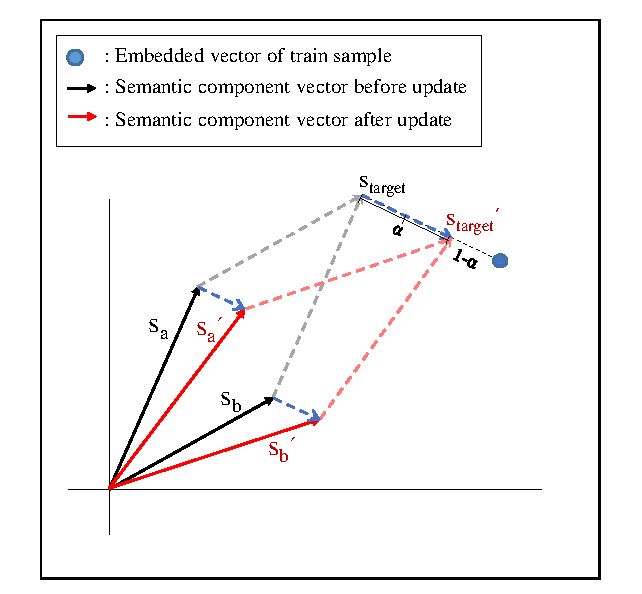
\includegraphics[width=\columnwidth]{../../figures/update.pdf}
  \caption{The semantic components are updated so that $ \mathbf{s}_{\text{target}} $ is close to the embedding vector. When updating, we divide difference vector between $\mathbf{s}_{\text{target}}$ of current step and embedding vector equally and we add it to each semantic component vectors, such that $\mathbf{s}_{\text{target}}$ of next step to be locate at Internally dividing point of current $\mathbf{s}_{\text{target}}$ and embedding vector of sample. 
}
  \label{fig:update}
\end{figure}



\begin{algorithm}[!htb]%centerloss
\SetAlgoNoLine
\SetKwFunction{Ftarget}{getTargetSemanticVectors}
\SetKwFunction{Fnew}{getNewSemanticComponentVectors}

\KwIn{Extracted handcrafted features of training data $v_i$ and their semantic components $\mathbf{y}_i$. Initialized parameters $\theta$ in neural embedder. parameters $W, b$ in classifier. initialized semantic component vectors $\mathbf{s}$.Importance coefficients $\textbf{c}$. Hyperparameter $\lambda$, $\alpha$, learning rate $\mu$. }
\KwOut{The parameters $\theta$, $W$, $b$ }
\Repeat{converge}{
    $s_\text{target} = \Ftarget(s_{\mathbf{y}})$ \\
	Compute total loss by $L = L_s + \lambda L_c$\\
	Update parameters $\theta$ by $\theta \leftarrow \theta - \mu \frac{\partial L}{\partial\theta}$ \\
	Update parameters $W$ by $W \leftarrow W - \mu \frac{\partial L}{\partial W}$\\
	Update parameters $b$ by $b \leftarrow b - \mu \frac{\partial L}{\partial b}$\\	
	Update semantic component vectors $s$ by $s \leftarrow \Fnew()$
	

	}
	\caption{The semantics-aware representation vector learning algorithm. }
\label{alg:centerloss}
\end{algorithm}





\begin{algorithm}[!htb]%functions
  \SetAlgoNoLine
  \DontPrintSemicolon
  \SetKwFunction{Ftarget}{getTargetSemanticVectors}
  \SetKwFunction{Fnew}{getNewSemanticComponentVectors}
  
  \SetKwProg{Fn}{Function}{:}{}
  \Fn{\Ftarget{$\mathbf{s}$}}{
    $M \leftarrow $ The number of semantic components \\
  	
    
	\If{Summation Model}
	{$s_{\text{target}} \leftarrow \sum_i^M{s_i}$}
	\ElseIf{Average Model}
	{$s_{\text{target}} \leftarrow \frac{1}{M}\sum_i^M{s_i}$}    
    
    \KwRet $s_{\text{target}}$\;
  }
  \;
    
  \SetKwProg{Pn}{Function}{:}{}
  \Pn{\Fnew{$\mathbf{s}$, $s_{\text{target}}$, $e$, $\alpha$, $\mathbf{c}$}}{
    $M \leftarrow $ The number of semantic components \\
    \ForEach{$i \in \{1, 2, ..., C\}$}{
	  \If{Summation Model}
	  {$s_i \leftarrow s_i - \frac{\alpha}{M}(s_{\text{target}} - e)$}
	  \ElseIf{Average Model}
	  {$s_i \leftarrow s_i - \alpha (s_{\text{target}} - e)$ }
	  \If{Weighted Model}
	  {$s_i \leftarrow \frac{s_i}{||s_i||} c_i$}    
    }
    \KwRet $\mathbf{s}$
  }
  \;  

  \caption{Definitions of functions. }
\label{func:functions}
\end{algorithm}

\section{Evaluation}
In this section, we evaluate the performance of our MR system in several ways, and verify that we have performed the semantic-aware malware retrieval task well.

\begin{table*}[!htb]%apk_result
\caption{APK19000 Querying Results}
\label{tab:apk_result}
\begin{minipage}{\textwidth}
\begin{center}
\begin{tabular}{|c|c|c|c|c|c|c|c|c|c|c|c|c|}
\hline
Dataset             & \multicolumn{6}{c|}{Querying trainset}                      & \multicolumn{6}{c|}{Querying validset}                      \\ \hline
Metric              & \multicolumn{3}{c|}{Precision}  & \multicolumn{3}{c|}{Weighted precision} & \multicolumn{3}{c|}{Precision}  & \multicolumn{3}{c|}{Weighted precision} \\ \hline
k              & top1   & top10  & top100 & top1      & top10     & top100   & top1   & top10  & top100 & top1      & top10     & top100   \\ \hline
Weighted centerloss (sum)  & 0.9846 & 0.9743 & 0.9374 & 0.9869    & \textbf{0.9802}   & \textbf{0.955}    & 0.8717 & 0.862  & 0.8272 & 0.8808    & 0.8746    & 0.8534   \\ \hline
Weighted centerloss (avg) & \textbf{0.9856} & 0.9772 & \textbf{0.9481} & 0.9855    & 0.9779    & 0.9528   & \textbf{0.8929 }& \textbf{0.8837 }& 0.8559 & \textbf{0.8893   } & 0.8815    & 0.8591   \\ \hline
Centerloss (sum)         & 0.9843 & 0.9737 & 0.9358 & 0.984     & 0.9733    & 0.9388   & 0.8736 & 0.8676 & 0.8373 & 0.8752    & 0.872     & 0.8462   \\ \hline
Centerloss (avg)        & 0.987  & \textbf{0.9776} & 0.9474 & 0.9872    & \textbf{0.9776}    & 0.9472   & 0.8845 & 0.8779 & \textbf{0.8562} & 0.8892    & \textbf{0.8829}    & \textbf{0.8631}   \\ \hline
Multi-label (baseline2)               & 0.9764 & 0.9617 & 0.9115 & 0.9752    & 0.9593    & 0.9094   & 0.8871 & 0.8713 & 0.8184 & 0.8869    & 0.8704    & 0.8236   \\ \hline
Single-label (baseline1)              & 0.9035 & 0.8727 & 0.8061 & 0.9004    & 0.8667    & 0.7946   & 0.8489 & 0.8231 & 0.7446 & 0.8434    & 0.8151    & 0.733    \\ \hline
\end{tabular}
\end{center}
\bigskip\centering
\end{minipage}
\end{table*}%


\begin{table*}[!htb]%pe_result
\caption{PE1300 Querying Results}
\label{tab:pe_result}
\begin{minipage}{\textwidth}
\begin{center}
\begin{tabular}{|c|c|c|c|c|c|c|c|c|c|c|c|c|}
\hline
Dataset             & \multicolumn{6}{c|}{Queyring trainset}                      & \multicolumn{6}{c|}{Queyring validset}                      \\ \hline
Metric              & \multicolumn{3}{c|}{precision}  & \multicolumn{3}{c|}{weighted precision} & \multicolumn{3}{c|}{precision}  & \multicolumn{3}{c|}{weighted precision} \\ \hline
k              & top1   & top10  & top100 & top1      & top10     & top100   & top1   & top10  & top100 & top1      & top10     & top100   \\ \hline
Weighted centerloss (sum)  & 1      & 1      & 0.9487 & 1         & 1         & 0.9329   & 0.9082 & 0.9075 & 0.8875 & 0.8816    & 0.881     & 0.8547   \\ \hline
Weighted centerloss (avg) & 1      & 1      & \textbf{0.9613} & 1         & 1         & \textbf{0.9671}   & \textbf{0.9203} & \textbf{0.9186} & \textbf{0.9029 }& \textbf{0.9142}    &\textbf{ 0.9085}    & \textbf{0.8916}   \\ \hline
Centerloss (sum)         & 1      & 1      & 0.9483 & 1         & 1         & 0.9319   & 0.9058 & 0.9058 & 0.8839 & 0.8845    & 0.8845    & 0.8487   \\ \hline
Centerloss (avg)        & 1      & 1      & 0.9544 & 1         & 1         & 0.965    & 0.9179 & 0.9179 & 0.8999 & 0.9048    & 0.9048    & 0.888    \\ \hline
Multi-label (baseline2)               & 0.9877 & 0.9665 & 0.7949 & 0.9877    & 0.9668    & 0.7793   & 0.8913 & 0.8894 & 0.8033 & 0.8666    & 0.8676    & 0.7692   \\ \hline
Single-label (baseline1)              & 0.9647 & 0.9004 & 0.7397 & 0.9608    & 0.8961    & 0.7235   & 0.8865 & 0.8597 & 0.7805 & 0.8784    & 0.8413    & 0.7501   \\ \hline
\end{tabular}
\end{center}
\bigskip\centering

\end{minipage}
\end{table*}%


\subsection{Implementation and Setup}
\textbf{Datasets. } 
The dataset used for learning and evaluation of the model is composed of samples crawling from VirusTotal\cite{total2012virustotal} and certified by security expert. In addition, Labeling was automated from the detection results of dozens of AntiVirus engines provided by VirusTotal. The detection results of each AntiVirus engine in VirusTotal are parsed in a meaningful word tokens, and the security expert selected labels from the word tokens. In addition, labels were prioritized according to their importance. This saves the time of the security expert in labeling the malware samples, while achieving accurate labels. Finally, for one sample, we have two types of labels: a representative label and a multi-label. The multi-label includes a representative label. Among the datasets, train set and test set were randomly sampled by 7: 3. And the distribution of samples over the representative label is even.

\begin{itemize}
	\item{ \textbf{Dataset 1. PE1300. } Among the more than 50,000 PE samples crawled from VirusTotal, the security expert verified about 2,000 PE samples with 10 labels. Four of the labels are representative labels and the number of samples for the representative label is almost the same.
	}
	\item{ \textbf{Dataset 2. APK19000. } In the case of APK, there are 19,000 samples from 190,000 samples crawled by VirusTotal, which were verified by expert, and used 83 kinds of labels. Of these, 19 labels are representative labels, and the number of samples for each representative label is 1000.
	}
\end{itemize}

\textbf{Settings. }

The feature extracter module extracts the malware image feature \cite{nataraj2011malware} and resize it to 224 by 224.
The network structure of the neural embedder module is convolutional neural netowrk which has five convolutional layers and two fully connected layers using batch normalization \cite{ioffe2015batch}. The previous layer of the last layer used leaky relu\cite{xu2015empirical} as activation function and the rest of the activation function are relu \cite{nair2010rectified}. 
The malware image \cite{nataraj2011malware} is passed through neural embedder. The convolutional layers extract features to contain local shift invariant characteristics of the malignant region or the region that characterizes the malware.

The hyper parameters used in the experiment are as follows. Adam optimizer\cite{kingma2014adam} was used as the optimizer and the learning rate was 0.001. $\alpha$ in centerloss is 0.1. When learning the PE1300 dataset, we used 0.1 as $\lambda$, which is the ratio of cross-entropy loss and centerloss, and 0.001, when learning APK19000. 


\textbf{Models. }
There are six models used in the experiment. First, the single-label model is a first baseline of our experiments, in which the auxiliary task classifies representative label using softmax-cross-entropy as a loss function. The multi-label model is a deep learning model designed to classify multiple labels into multi-task learning using a sigmoid cross-entropy as a loss function. This is a second baseline of our experiment. Next, to find out the effect of applying centerloss, we added centerloss to the multi-label model. There are two models that combine semantic components as average and summation. And to see the effect of scoring, here is the weighted center loss model with the importance coefficient added as a constraint. This method also has two versions of average and summation models.
  

\begin{table*}[!htb]%class_variances
\caption{Class Variances}
\label{tab:class_variances}
\begin{minipage}{\textwidth}
\begin{center}
\begin{tabular}{|c|c|c|c|c|c|c|}
\hline
Dataset             & \multicolumn{3}{c|}{APK19000}                               & \multicolumn{3}{c|}{PE1300}                                             \\ \hline
Variance              & Intra-class  & Inter-class  & Inter/Intra & Intra-class  & Inter-class  & Inter/Intra  \\ \hline
Weighted centerloss (sum)  & 0.0473              &         2.793       &     59.0486             & 0.129               &              2.169 &              16.8140    \\ \hline
Weighted centerloss (avg) & \textbf{0.0101}              &          \textbf{    1.1906} &    \textbf{117.8812 }            & \textbf{0.0361             } &                   \textbf{ 1.2698} &      \textbf{35.1745}                   \\ \hline
Centerloss (sum)         & 0.2268              &                    5.2967 &          23.3541               & 0.1748              &              1.8299       &    10.4685                     \\ \hline
Centerloss (mean)        & 0.0258              &                    1.2785 &           49.5543              & 0.1332              &        1.6826             &     12.6321                    \\ \hline
Multi-label (baseline2)               & 2.4956              &                    21.8435 &       8.7528                    & 25833.582           &        840.54             &        0.0325               \\ \hline
Single-label (baseline1)              & 1.2103              &                    15.18 &            12.5423             & 2310.7649           &      267.683               &           0.1158              \\ \hline
\end{tabular}
\end{center}
\bigskip\centering
\end{minipage}
\end{table*}%


\begin{table}[!htb]%auxiliary_result 
\caption{Auxiliary Task Results}
\label{tab:auxiliary_result}
\begin{minipage}{\columnwidth}
\begin{center}
\begin{tabular}{|c|c|c|}
\hline
Dataset             & APK19000 & PE1300 \\ \hline
Weighted center (sum)  & 0.9618   & 0.9801 \\ \hline
Weighted center (avg) & 0.9636   & \textbf{0.9812} \\ \hline
Centerloss (sum)         & \textbf{0.9728 }  & 0.9753 \\ \hline
Centerloss (avg)        & 0.9705   & 0.9574 \\ \hline
Multi-label(baseline2)          & 0.9606   & 0.9495 \\ \hline
Single-label(baseline1)              & 0.9508   & 0.946  \\ \hline
\end{tabular}
\end{center}
\bigskip\centering
\end{minipage}
\end{table}%


\subsection{Querying Quantitative Test}

In this part, we will analyze the effect of centerloss by comparing precision at top K value obtained by querying with malware samples for each model and class variance of representation vectors.

\textbf{Metrics. } The metrics used in quantitative evaluation are as follows. We used precision to evaluate the performance of MR system, weighted precision to evaluate scoring, and intra and inter class variance.

\begin{itemize}
	\item{ \textbf{Precision} 
	
	Let the labels of the querying sample $q$ be $y_{q_1}, y_{q_2}, ..., y_{q_m}$. Let the labels of the $k$ search result samples $r_1, r_2, ..., r_k$ obtained from Ranking module $R$ be $y_{r_1}, y_{r_2}, ..., y_{r_l}$ respectively . In this case, precision at top K is obtained as follows.

	\[
	Precision_{K} = \frac{1}{N} *\sum_{i=1}^{N}{ \frac{ \sum_{k=1}^{K}{|Y_{q_i} \cap Y_{r_k}|}}{  \sum_{k=1}^{K}{ |Y_{r_k}| }  }}
	\]\\
	where $|Y|$ is the number of elements of set $Y$.
	}
	\item{ \textbf{Weighted precision} 
	
	Weighted precision is calculated in the same way as precision, adding weighted importance coefficients of each label. This metric provides better results when model hits important labels.

	\[
	WeightedPrecision_{K} = \frac{1}{N} *\sum_{i=1}^{N}{ \frac{ \sum_{k=1}^{K}{|Y_{q_i} \cap Y_{r_k}|_w}}{  \sum_{k=1}^{K}{ |Y_{r_k}|_w }  }}
	\]\\
	where $|Y|_w = \sum_i{c_{y_i}}$ and $c_j$ is importance coefficient of j'th label.
	}
	\item{ \textbf{Inner class variance} 
	
	Inner class variance represents the variance of the representation vector of samples in the same class. That is, it is a metric that measures how much the same classes are gathered together. Because our samples have a multi-label, we measure the variance for a sample with the same label combination and average it.
  
	}
	\item{ \textbf{Inter class variance} 
	
	Inter class variance is a metric that indicates how far apart other classes are. Likewise, the distances between sample vectors with different label combinations were measured and average it.
 
	}
	%\item{ \textbf{inter class variance over inner class variance} 
	%inter cliass variance 대비 inner class variance 를 측정하여 여러 모델의 임베딩 벡터 셋들이 얼마나 IR 이 잘 비교할 수 있게 된다.}
\end{itemize}



\textbf{Sample querying results. }
From the results of Table. \ref{tab:apk_result} and Table. \ref{tab:pe_result}, we were able to observe the following. First, the precision is better than the multi-label baseline model when using centerloss. Especially, as the K increases, precision value of the multi-label baseline model falls sharply, but the centerloss models do not. Second, the models with the importance coefficient added to the centerloss have better weighted precision results than the other models. Finally, we observed that using average as a combination of semantic components was slightly better than using summation method.

From the above experiments, we can confirm that the above quantitative values ​​are generally higher when the MR system is constructed using multi-label centerloss. This shows that the semantic understanding attribute of desired property of the MR system is more satisfactory than the other methods. We also showed that scoring is possible in MR systems using weighted centerloss with deep learning.

\textbf{Class variances. }
We measured the class variance to determine the cause of the above results. The results can be seen in the Table. \ref{tab:class_variances}. From this result, we confirmed that using centerloss reduces the inner-class variance. In addition, to measure the relative class variance of the models, the intra-class variance and the inter-class variance of the embedding vectors were measured and compared. The larger the value of the inter-class variance / intra-class variance is, the more discriminative the representation vectors are, meaning that retrieval results may be better.

\textbf{Auxiliary task results. }
Table.\ref{tab:auxiliary_result} represents the AUC for the validation set of the auxiliary task.The purpose of the original Auxiliary task is literally a subtask to learn the representation vector to be used in the MR system, but with the centerloss, we can see a slight performance improvement.


\subsection{Querying Qualitative Test}
In this part, we list the top k results obtained by querying the MR system we built in the three ways introduced in Section 4.1. Thus, our proposal shows that the performance of the MR system has improved. For each querying test, we can see the querying method in the Figure. \ref{fig:qualitative_all}.

\textbf{Querying by malware sample. }
A sample of the APK malware with a semantic component consisting of \texttt{agent}, \texttt{slocker}, \texttt{jisut}, and \texttt{ransom} was queried to the learned MR system with the models described above. The retrieval result can be observed in Table.\ref{tab:sample_query_result}. The system learned by the centerloss (add) model is better than the other two models.
\[
   query = \mathbf{e_q} 
\]


% Table
\begin{table*}%sample_query_result
\caption{Queyring by sample}
\label{tab:sample_query_result}
\begin{minipage}{\textwidth}
\begin{center}
\begin{tabular}{@{}lllll@{}}
\toprule
\multicolumn{1}{c}{Semantics of queried sample}   & Top & \multicolumn{1}{c}{Centerloss (sum)} & \multicolumn{1}{c}{Multi-label}     & \multicolumn{1}{c}{Single-label}             \\ \midrule
\multicolumn{1}{c}{agent, slocker, jisut, ransom} & 1   & agent, slocker, jisut, ransom  & agent, slocker, jisut, ransom & slocker, jisut, ransom                 \\
                                                  & 2   & agent, slocker, jisut, ransom  & agent, slocker, jisut, ransom & slocker, jisut, ransom                 \\
                                                  & 3   & agent, slocker, jisut, ransom  & agent, slocker, jisut, ransom & slocker, jisut, ransom                 \\
                                                  & 4   & agent, slocker, jisut, ransom  & agent, slocker, jisut, ransom & dropper, agent, slocker, jisut, ransom \\
                                                  & 5   & agent, slocker, jisut, ransom  & agent, slocker, jisut, ransom & slocker, jisut, ransom                 \\
                                                  & 6   & agent, slocker, jisut, ransom  & agent, slocker, jisut, ransom & dropper, agent, slocker, jisut, ransom \\
                                                  & 7   & agent, slocker, jisut, ransom  & slocker, jisut, ransom        & slocker                                \\
                                                  & 8   & agent, slocker, jisut, ransom  & agent, slocker, jisut, ransom & slocker, jisut, ransom                 \\
                                                  & 9   & agent, slocker, jisut, ransom  & slocker, jisut, ransom        & agent, slocker, jisut, ransom          \\
                                                  & 10  & agent, slocker, jisut, ransom  & slocker, jisut, ransom        & slocker, jisut, ransom                 \\ \bottomrule
\end{tabular}
\end{center}
\bigskip\centering
\end{minipage}
\end{table*}%

\textbf{Querying by semantic components. }
The next test is to querying the semantic components and retrieve samples. We tested the APK MR system learned by the centerloss (add) model. We used the sum of the semantic component vectors corresponding to \text{agent}, \text{ewind}, and \text{downloader} as a query.
\[
   query = \mathbf{s}_{\text{agent}} + \mathbf{s}_{\text{ewind}} + \mathbf{s}_{\text{downloader}}  
\]
Results can be found in Table.\ref{tab:semantics_query_result}. In our learning data set, there are 89 samples consisting of \text{agent}, \texttt{ewind}, and \texttt{downloader}. We could see that these samples were all searched in the samples up to the top 90.

% Table
\begin{table*}%semantics_query_result
\caption{Quering by semantics}
\label{tab:semantics_query_result}
\begin{minipage}{\textwidth}
\begin{center}
\begin{tabular}{@{}lcl@{}}
\toprule
\multicolumn{1}{c}{\begin{tabular}[c]{@{}c@{}}Queried semantic components\end{tabular}} & Top        & \multicolumn{1}{c}{Centerloss (sum)} \\ \midrule
\multicolumn{1}{c}{\begin{tabular}[c]{@{}c@{}}agent, ewind,  downloader\end{tabular}}    & 1$\sim$86  & agent, ewind, downloader            \\
                                                                                           & 87         & agent, ewind, downloader, ransom    \\
                                                                                           & 88$\sim$90 & agent, ewind, downloader            \\
                                                                                           & 91         & agent, ewind, downloader, ransom    \\
                                                                                           & 92         & agent, ewind, downloader, ransom    \\
                                                                                           & 93         & downloader, agent, ewind, fakeinst  \\
                                                                                           & 94         & ewind, downloader                   \\ \bottomrule
\end{tabular}
\end{center}
\bigskip\centering
\end{minipage}
\end{table*}%


\textbf{Querying by the combination of semantics and sample. }
Finally, we tested to add or subtract some semantic components to the malware samples for querying. As in the previous two experiments, we tested for APK. The APK samples used in the experiment have four semantic components: \texttt{smsreg}, \texttt{agent}, \texttt{smspay}, \texttt{smssend}. Among these samples, the \texttt{smssend} component was omitted and the \texttt{dropper} component was added to create the query statement.
\[
   query = \mathbf{e_q} - \mathbf{s}_{\text{smssend}} + \mathbf{s}_{\text{dropper}} 
\]
In our learning data set, there are 56 samples consisting of four semantic components of \texttt{smsreg}, \texttt{agent}, \texttt{smspay}, and \texttt{dropper}, and all the samples are found in top 69 results.


% Table
\begin{table*}%sample_and_semantics_query_result
\caption{Querying by the combination of semantics and sample}
\label{tab:sample_and_semantics_query_result}
\begin{minipage}{\textwidth}
\begin{center}
\begin{tabular}{llcl}
\hline
\multicolumn{2}{c}{Query}                                                                    & \multirow{2}{*}{Top} & \multicolumn{1}{c}{\multirow{2}{*}{Centerloss (sum)}} \\
\multicolumn{1}{c}{Sample}                         & \multicolumn{1}{c}{Semantic components} &                      & \multicolumn{1}{c}{}                                 \\ \hline
\multicolumn{1}{c}{smsreg, agent, smspay, smssend} & - smssend + dropper                     & 1$\sim$34            & smsreg, dropper, agent, smspay                       \\
                                                   &                                         & 35                   & smsreg, dropper, smspay                              \\
                                                   &                                         & 36$\sim$45           & smsreg, dropper, agent, smspay                       \\
                                                   &                                         & 46                   & mobilepay, smsreg, dropper,agent, smspay             \\
                                                   &                                         & 47$\sim$49           & smsreg, dropper, agent, smspay                       \\
                                                   &                                         & 50                   & smsreg, dropper, agent, smspay, dowgin               \\
                                                   &                                         & 51                   & smsreg, dropper, agent, smspay                       \\ \hline
\end{tabular}
\end{center}
\bigskip\centering
\end{minipage}
\end{table*}%

%
%\subsection{Generalization}
%입력 Feature 가 Semantics-aware feature 일 수록 새로운 샘플에 대한 Error 가 더 작다. 우리가 제안한 목적함수는 멀티 레이블과 레이블 별 중요도로부터 해당 샘플이 시멘틱 스페이스에서 어디에 위치해야하는지를 가이드해준다. 따라서 Train Samples 에 대해서는 데이터의 입력 Feature가 Semantic-aware 하지 않더라도 원하는 곳에 특징 표현 벡터를 위치시킬 수 있다. 하지만 새로 보는 샘플의 representation vector 가 우리가 원하는 곳에 위치하게 된다는 보장은 없다. 딥러닝의 하이러키컬 특징 표현 학습이 MWC loss 를 통해 가이드 되는 Semantic을 학습할 수 있도록 하려면 입력 Feature가 충분히 Semantics-aware 해야 하고, 이에 관련된 연구들은 섹션2에서 소개하였다. 
%
%우리는 이 차이를 보이기 위해 semantics-aware level 이 다른 두 가지 피쳐에 대해 벡터 표현을 학습시키고, validation set 의 벡터 표현이 Semantic space 위에 잘 위치하는지 확인하는 실험을 한다. 첫 번째 실험에 사용되는 피쳐는 간단한 정적 분석을 통해 얻을 수 있는 Size, entropy\citep{} 이고, 두 번째 실험에 사용되는 피쳐는보다 조금 더 Semantics-aware 한 피쳐인 Thumbnail\citep{} 이다. 위에서 진행한 정량 평가와 정성 평가를 두 실험에 대해 진행해 본 결과 더 semantics-aware한 피쳐를 입력으로 사용할 수록 평가의 결과가 좋았고 이는 즉 Generalization 이 더 된다는 것을 의미한다. 즉, 누구라도 더 Semantics-aware한 피쳐를 입력으로 넣어줄 수 있다면, 간단히 Add-on 가능한 MWC loss 를 사용하여 훌륭한 Semantic space 를 구축할 수 있게 된다. 

% 시간이 된다면 APK Call-graph 도... 하면 좋을텐데..  


\section{Future Works}

현재 방법은 멀티 레이블이 다 정확해야 한다. 아니라면 모델이 noise 로부터 오해를 쉽게 한다. 하지만 이 도메인에서 정확한 레이블을 얻기란 쉽지 않다. 따라서 label noise-robust MLC 를 만들어 멀웨어의 feature 로부터 멀웨어 샘플의 리얼 레이블을 denoising 을 통하여 추정하고, 이를 통해서 IR 시스템을 만든다면 더 semantic-aware 한 Malware Information System 을 만들 수 있을 것이라 추정된다.
더불어 새로운 샘플에 대한 빠른 대응도 IR 시스템에서 중요한 부분인데, 딥러닝 모델이다보니 학습해야할 시간이 필요하다. continual learning 혹은 online update 를 사용해서 이를 해결하는 것도 우리의 Future work이다. 



\section{Related Works}


Nataraj et al. \cite{nataraj2013sarvam} proposed a large scale malware search and retrieval system. In this paper, he proposes a method to retrieve fingerprints from malware image and retrieves similar samples through nearest neighbor search. Upchurch et al. \cite{upchurch2015variant} introduced a framework for detecting variant malware through similarity testing. This framework extracted the static features using BitShred, TLSH, sdhash, ssdeep, and compared them to determine whether they were similar malware. Palahan et al. \cite{palahan2013extraction} proposed a method of comparing similarities between malware by extracting significant malicious behaviors from the system call dependency graph and comparing them. Several neural IR models have been proposed in the document retrieval domain, and many models have been studied to obtain a good representation of text\cite{mitra2017learning,cohen2016end,huang2013learning}.

 Chih-Kuan et al. \cite{yeh2017learning} trained Canonical Correlated AutoEncoder models using label-correlation sensitive loss function as a way to obtain multilabel embedding. In this paper, he showes that the relationship between labels with dependency is trained end-to-end and solves the multi-label classification task, and proved to be effective for missing label problem of multilabel classification.

\section{Conclusions}

우리는 딥러닝을 활용하여 멀웨어 리트리벌 시스템을 만드는 데에서 생겼던 문제들을 새로운 로스를 정의함으로써 해결했다. 특히 기존 방법들보다 [제너럴라이제이션] 측면에서 좋다는 것을 정량적, 시각적으로 증명했다. 이는 수많은 보안 전문가들의 업무 코스트를 낮춰줄 수 있을 것이라 믿는다.

\appendix

\section{Location}

Note that in the new ACM style, the Appendices come before the References.


\begin{acks}
% TODO: For the submission, don't include acknowledgments since they would most likely deanonymize you.
\end{acks}
